\documentclass[border=10pt]{standalone}

\usepackage{tikz}
\usepackage{tikzsymbols}
\usetikzlibrary{calc,patterns,shapes.geometric}

\def\centerarc[#1](#2)(#3:#4:#5){\draw[#1] ($(#2)+({#5*cos(#3)},{#5*sin(#3)})$) arc (#3:#4:#5);}

\begin{document}
	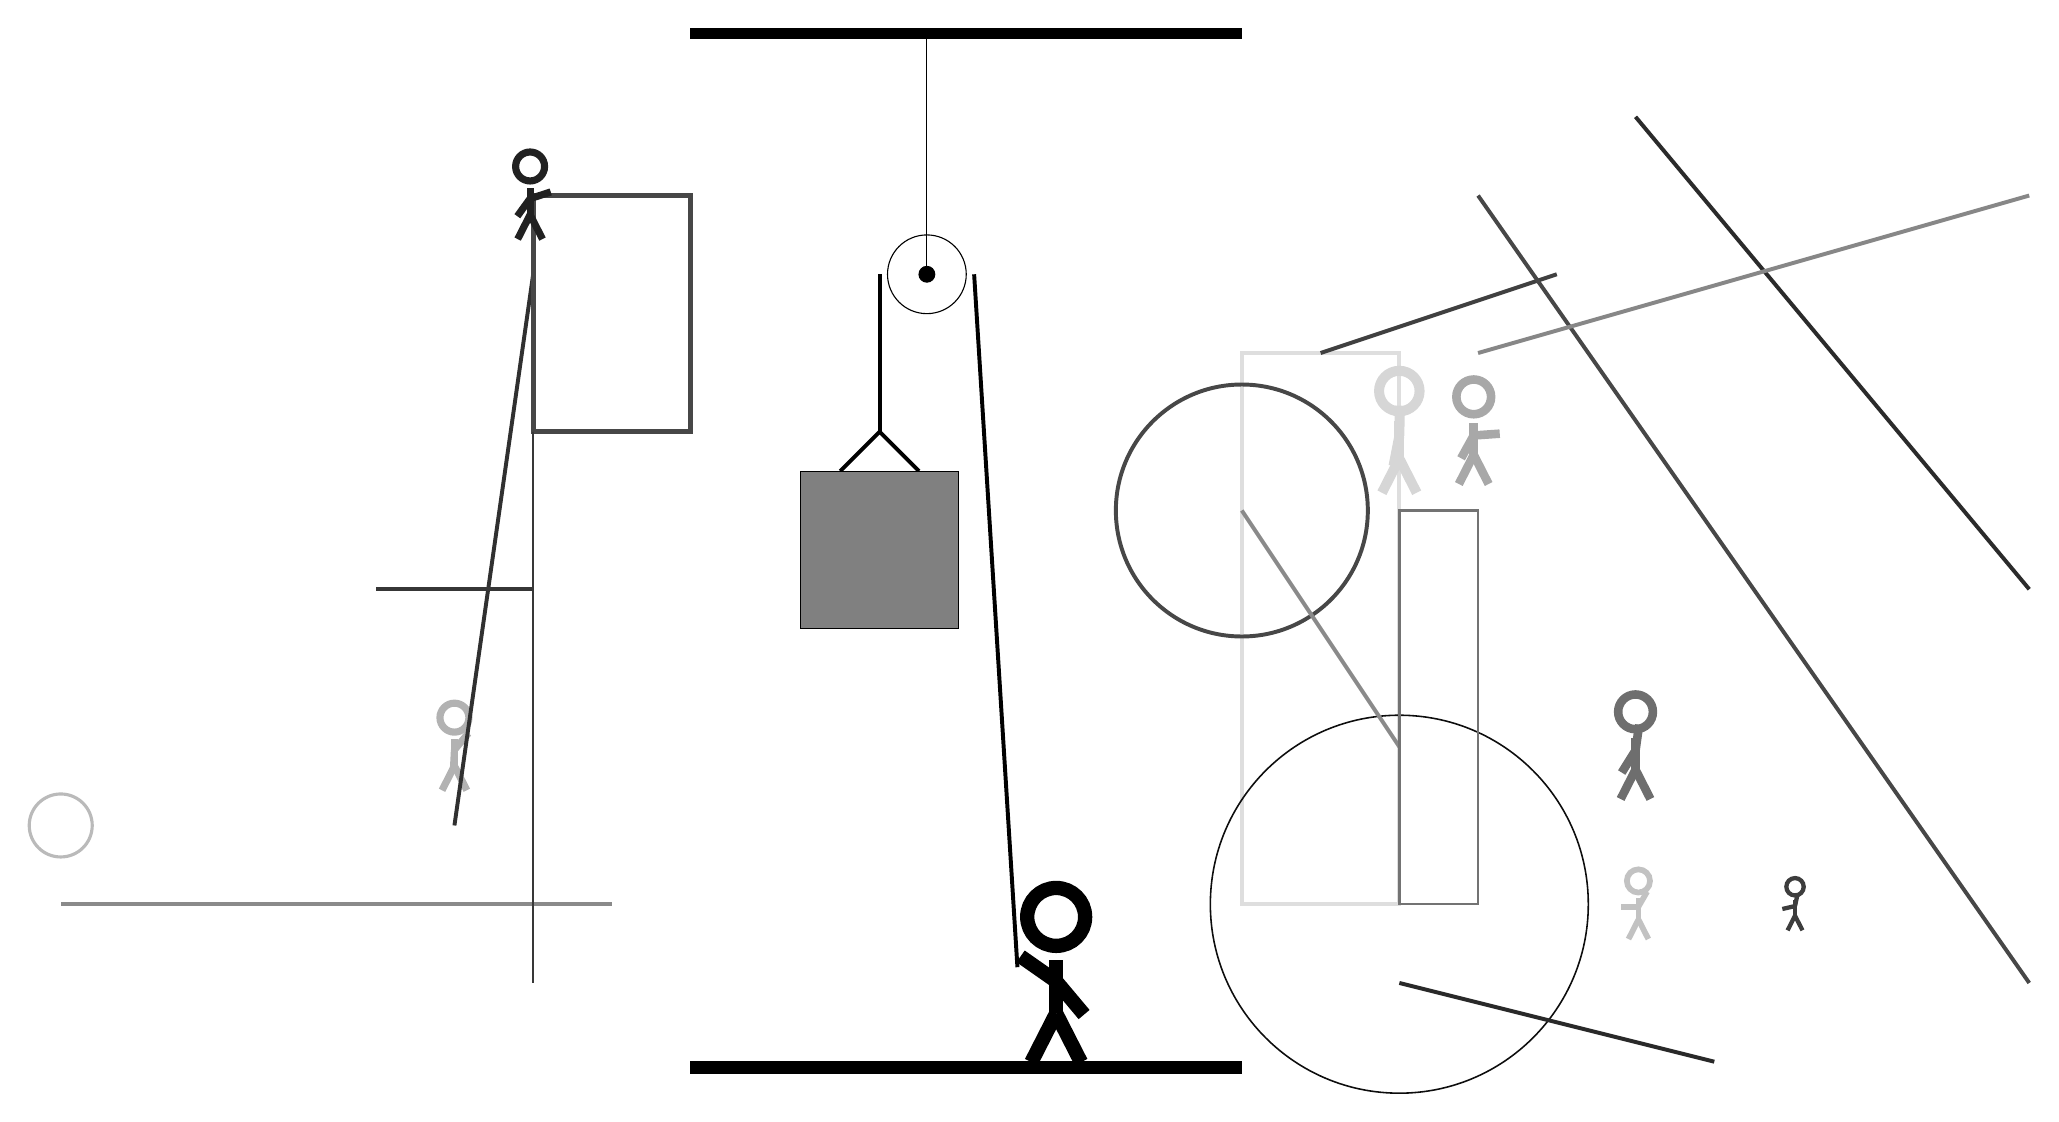
\begin{tikzpicture}
		%%%%% START %%%%%
		
		\draw[fill=black] (-2, 10) rectangle (5, 10.125);
		
		\draw (1, 7) circle (0.5);
		\draw[fill=black] (1, 7) circle (0.1);
		\draw (1, 10) -- (1, 7);
		
		\node[line width=0.2mm, color=black!30] at (-5, 1) {\Strichmaxerl[5][87][50]};
		
		\draw[line width=0.5mm, color=black!13] (5, -1) rectangle (7, 6);
		\draw[line width=0.5mm, color=black!81](-5, 0) -- (-4, 7);
		\node[line width=0.7mm, color=black!24] at (10, -1) {\Strichmaxerl[4][0][60]};
		\node[line width=0.4mm, color=black!16] at (7, 5) {\Strichmaxerl[7][79][89]};
		
		\draw [line width=0.5mm, color=black!72](5, 4) circle (1.6);
		
		\node[line width=0.7mm, color=black!76] at (12, -1) {\Strichmaxerl[3][13][78]};
		
		\draw[line width=0.5mm, color=black!75](6, 6) -- (9, 7);
		\draw[line width=0.6mm, color=black!72] (-4, 8) rectangle (-2, 5);
		\draw [line width=0.2mm, color=black!95](7, -1) circle (2.4);
		\draw[line width=0.5mm, color=black!72](8, 8) -- (15, -2);
		\node[line width=0.3mm, color=black!57] at (10, 1) {\Strichmaxerl[6][58][82]};
		\draw [line width=0.4mm, color=black!27](-10, 0) circle (0.4);
		\draw[line width=0.5mm, color=black!79](-4, 3) -- (-6, 3);
		\draw[line width=0.5mm, color=black!46](-3, -1) -- (-10, -1);
		\draw[line width=0.2mm, color=black!78] (-4, -2) rectangle (-4, 5);
		
		\draw[line width=0.5mm, color=black!83](10, 9) -- (15, 3);
		\node[line width=0.6mm, color=black!34] at (8, 5) {\Strichmaxerl[6][61][4]};
		\draw[line width=0.5mm, color=black!47](8, 6) -- (15, 8);
		\draw[line width=0.5mm, color=black!46](5, 4) -- (7, 1);
		\draw[line width=0.3mm, color=black!55] (7, -1) rectangle (8, 4);
		
		\draw[line width=0.5mm, color=black!84](7, -2) -- (11, -3);
		\node[line width=0.2mm, color=black!87] at (-4, 8) {\Strichmaxerl[5][54][18]};
		
		\draw[line width=0.5mm] (-0.1, 4.5) -- (0.4, 5.0) -- (0.9, 4.5);
		\draw[fill=black!50] (-0.6, 4.5) rectangle (1.4, 2.5);
		
		\draw[line width=0.5mm] (0.4, 7) -- (0.4, 5.0);
		\centerarc[line width=0.5mm](1, 7)(0:180:0.6);
		\draw[line width=0.5mm](1.6, 7) -- (2.15, -1.8);
		
		\node at (2.6, -1.9) {\Strichmaxerl[10][-35][-50]};
		
		\draw[fill=black] (-2, -3) rectangle (5, -3.15);
		
		%%%%% END %%%%%
	\end{tikzpicture}
\end{document}